\documentclass[tikz]{standalone}

\usepackage{pgfplots}
\pgfplotsset{compat=1.16}

\begin{document}
        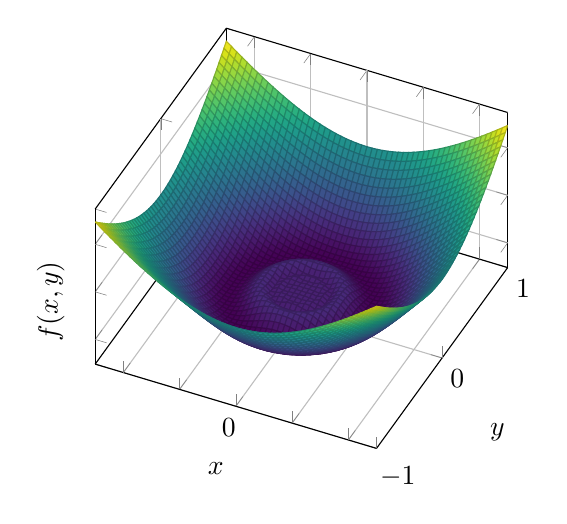
\begin{tikzpicture}
            \begin{axis}[
                colormap name=viridis,
                % 3d box,
                width=11cm,
                view={25}{40},
                axis equal image,
                % enlargelimits=false,
                grid=major,
                domain=-0.5:0.5,
                samples=55,
                yticklabels={,$-1$,$0$,$1$},
                xticklabels={,,,$0$},
                zticklabels={,,},
                xlabel=$x$,
                ylabel=$y$,
                zlabel={$f(x, y)$},
                ]
                \addplot3 [y domain = -0.5:0.5, surf]
                    {(x*x+y*y)*sin(deg(1/sqrt(x*x+y*y)))};
            \end{axis}
        \end{tikzpicture}
\end{document}
